\section{Precle} % (fold)
Precle pojawiły się po raz pierwszy w~książce Reidemeistera z~1932 roku jako przykład węzła o~trywialnym wielomianie Alexandera.

\label{sec:pretzel}
\begin{definition}
    \index{splot!Montesinosa}
    Splotem Montesinosa nazywamy splot o~poniższym diagramie
    kodowanym wymiernymi liczbami $\alpha_i/\beta_i$ oraz całkowitą $e$.
    Odpowiadają one supłom.
    \[
    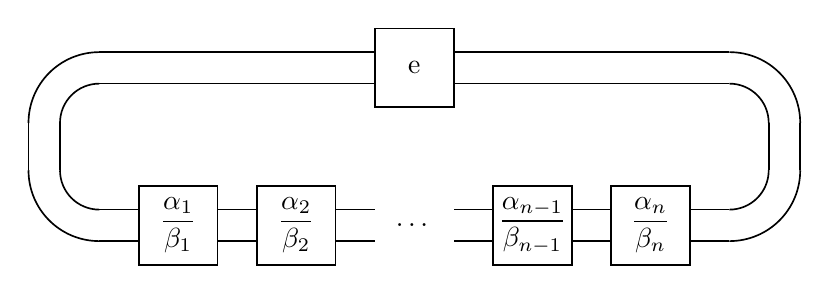
\begin{tikzpicture}[baseline=-0.65ex, scale=0.1]
    %\useasboundingbox (-5, -9) rectangle (5, 5);
        \draw[semithick] (-5, 5) rectangle (5, 15);
        \foreach \x in {0,1,3,4} {
            \draw[semithick] (15*\x-35, -15) rectangle (15*\x-25, -5);
        }
        \foreach \x in {0,1,2,3,4,5} {
            \draw[semithick] (15*\x-35, -8) to (15*\x-40, -8);
            \draw[semithick] (15*\x-35, -12) to (15*\x-40, -12);
        }
        \draw[semithick] (-40, -8) [in=down, out=left] to (-45, -3);
        \draw[semithick] (-40, -12) [in=down, out=left] to (-49, -3);

        \draw[semithick] (-40, 8) [in=up, out=left] to (-45, 3);
        \draw[semithick] (-40, 12) [in=up, out=left] to (-49, 3);

        \draw[semithick] (40, 8) [in=up, out=right] to (45, 3);
        \draw[semithick] (40, 12) [in=up, out=right] to (49, 3);

        \draw[semithick] (40, -8) [in=down, out=right] to (45, -3);
        \draw[semithick] (40, -12) [in=down, out=right] to (49, -3);

        \draw[semithick] (-45, -3)  to (-45, 3);
        \draw[semithick] (-49, -3)  to (-49, 3);
        \draw[semithick] (45, -3)  to (45, 3);
        \draw[semithick] (49, -3)  to (49, 3);

        \draw[semithick] (-5, 8)  to (-40, 8);
        \draw[semithick] ( 5, 8)  to ( 40, 8);
        \draw[semithick] (-5, 12)  to (-40, 12);
        \draw[semithick] ( 5, 12)  to ( 40, 12);

        \node at (0, 10) {e};
        \node at (0, -10) {\ldots};
        \node at (-15, -10) {$\displaystyle \frac{\alpha_2}{\beta_2}$};
        \node at (-30, -10) {$\displaystyle \frac{\alpha_1}{\beta_1}$};
        \node at (15, -10) {$\displaystyle \frac{\alpha_{n-1}}{\beta_{n-1}}$};
        \node at (30, -10) {$\displaystyle \frac{\alpha_n}{\beta_n}$};
    \end{tikzpicture}
    \]
\end{definition}

Klasyfikację splotów Montesinosa można znaleźć u~Burdego i~Zieschanga \cite{burde85}.

\begin{definition}
    \label{def:pretzel}
    \index{precel}
    Splot Montesinosa o~całkowitych współczynnikach nazywamy preclem.
\end{definition}

Na standardowym diagramie precla $(p_1, p_2, \ldots, p_n)$ występuje $p_1$ lewych skrzyżowań w~pierwszym suple, $p_2$ w~drugim, i~tak dalej.
Taki precel jest węzłem dokładnie wtedy, gdy $n$ oraz $p_i$ są nieparzyste lub dokładnie jedna z~liczb $p_i$ jest parzysta.

\begin{proposition}
    Jeśli co najmniej dwa współczynniki $p_i$ zerują się, splot jest rozdzielczy.
\end{proposition}

Nie jest prawdziwa implikacja odwrotna.

Precel $(1,1,1)$ to prawy trójlistnik, $(5, -1, -1)$ to węzeł dokerski $6_1$, $(-3, 0, -3)$ to splot dwóch trójlistników, zaś $(2p, 2q, 2r)$ (zapewne dla nieparzystych, różnych $p, q, r$) jest splotem trzech niewęzłów.
Precle $(-2, 3, 2n+1)$ są szczególnie użyteczne jako narzędzie do badania 3-rozmaitości.
Wiele twierdzeń, które dotyczą takich rozmaitości, opiera się na przykład na chirurgii Dehna precla $(-2, 3, 7)$.

Patrz także twierdzenie \ref{trotter}.
% Koniec sekcji Precle

Wielomian Alexandera precla $(p_1, \ldots, p_n)$ nie zależy od kolejności współczynników (jest to ćwiczenie 10.9 w~książce Livingstona).